\documentclass[10pt,conference]{IEEEtran}

\ifCLASSINFOpdf
	\usepackage[pdftex]{graphicx}
	%\graphicspath{{./figs/}}
	\DeclareGraphicsExtensions{.pdf,.jpeg,.png}
\else
	\usepackage[dvips]{graphicx}
	%\graphicspath{{./figs/}}
	\DeclareGraphicsExtensions{.eps}
\fi

\usepackage[cmex10]{amsmath}
\usepackage[tight,footnotesize]{subfigure}
\usepackage{xcolor}
\usepackage{float}
\usepackage[lined,ruled]{algorithm2e}

\usepackage[latin1]{inputenc}
\usepackage{tikz}
\usetikzlibrary{shapes}
\usetikzlibrary{arrows}

\usepackage[]{algorithm2e}

\newtheorem{property}{Property}
\newtheorem{proposition}{Proposition}
\newtheorem{theorem}{Theorem}
\newtheorem{conjecture}{Conjecture}
\newtheorem{question}{Question}
\newtheorem{definition}{Definition}
\newtheorem{corollary}{Corollary}

\makeatletter
\pgfdeclareshape{datastore}{
\inheritsavedanchors[from=rectangle]
\inheritanchorborder[from=rectangle]
\inheritanchor[from=rectangle]{center}
\inheritanchor[from=rectangle]{base}
\inheritanchor[from=rectangle]{north}
\inheritanchor[from=rectangle]{north east}
\inheritanchor[from=rectangle]{east}
\inheritanchor[from=rectangle]{south east}
\inheritanchor[from=rectangle]{south}
\inheritanchor[from=rectangle]{south west}
\inheritanchor[from=rectangle]{west}
\inheritanchor[from=rectangle]{north west}
\backgroundpath{
    %  store lower right in xa/ya and upper right in xb/yb
\southwest \pgf@xa=\pgf@x \pgf@ya=\pgf@y
\northeast \pgf@xb=\pgf@x \pgf@yb=\pgf@y
\pgfpathmoveto{\pgfpoint{\pgf@xa}{\pgf@ya}}
\pgfpathlineto{\pgfpoint{\pgf@xb}{\pgf@ya}}
\pgfpathmoveto{\pgfpoint{\pgf@xa}{\pgf@yb}}
\pgfpathlineto{\pgfpoint{\pgf@xb}{\pgf@yb}}
 }
}
\makeatother

\newcommand{\riham}[1]{{\color{red}{#1}}}
\newcommand{\james}[1]{{\color{blue}{#1}}}

\makeatletter
\newcommand{\removelatexerror}{\let\@latex@error\@gobble}
\makeatother
\newcommand{\myalgorithm}{%
	\begingroup
	\removelatexerror% Nullify \@latex@error
	\begin{algorithm*}[H]
		%...
	\end{algorithm*}
	\endgroup}


\begin{document}

\title{CS512 FUN Project - Spell Checking System}
\author{
\IEEEauthorblockN{Shengjie Li}
\IEEEauthorblockA{Rutgers University\\
	Piscataway, NJ, USA\\
Email: shengjie.li@rutgers.edu}
\and
\IEEEauthorblockN{Weikang Li}
\IEEEauthorblockA{Rutgers University\\
 Piscataway, NJ, USA\\
 Email: wl494@scarletmail.rutgers.edu}
\and
\IEEEauthorblockN{Junlin Lu}
\IEEEauthorblockA{Rutgers University\\
 Piscataway, NJ, USA\\
 Email: jl2364@scarletmail.rutgers.edu}
}

\maketitle
\begin{abstract}
\textnormal{
This article mainly introduces the achievement of a word spell checking system. This system is a handy tool for every user who wants to check whether there are errors in their text. In the system, we use a less memory-consuming version of trie --- ternary search tree for storing the dictionary. We use several methods including edit distance,  similarity keys, and n-grams to improve the accuracy of word correction suggestion. 
}
\end{abstract}
%\onecolumn \maketitle \normalsize \vfill

\IEEEpeerreviewmaketitle
%%%%%%%%%%%%%%%%%%%%%%%%%%%%%%%%%%%%%%%%%%%%%%%%%%%%%%%%%%%%%%%%%%%%%%%%%%%%%%%%%%%%%%%%%%%%%%%%%%%%%%%%%
\section{Project Description}\label{sec:1. Project Description}
%%%%%%%%%%%%%%%%%%%%%%%%%%%%%%%%%%%%%%%%%%%%%%%%%%%%%%%%%%%%%%%%%%%%%%%%%%%%%%%%%%%%%%%%%%%%%%%%%%%%%%%%%
\textnormal{
	The type of this project is implementation of an algorithm not covered in class.
 There are a lot of ways to detect spelling mistakes and correct the word. This system uses dictionary searching to detect possible correct spelling. Spelling checking plays an important part in our daily life, especially for international students whose mother language is not English, therefore developing a spell-checking system helps a lot and is extremely useful. 
We use a Trie to store the whole dictionary. More specifically, we use a ternary search tree, which is one kind of implementation of Trie. The correction of a word is a process of finding the most similar word. We achieve it using a combination of several methods like edit distance, similarity keys, and n-grams. Each one in our group is proficient in data structures and algorithms, so it is feasible for us to complete it within a semester. 
By avoiding some number of calculations and combining several different ways to calculate the difference between two words, we can somehow improve the efficiency and accuracy of this system. This is the novel part of this system.
We have not encountered any stumbling block yet. But we think the improvement of the accuracy of the spelling correction would be very hard after a certain point.
}

The project has four stages: Gathering, Design, Infrastructure Implementation, and User Interface.

%\subsection{Stage1 - The Requirement Gathering Stage. } \label{sec:1	Requirement Gathering Stage. } 
%
\begin{itemize} 
\item{The general description of this project's deliverables: } 
This project is a spell checking system which is able to detect spelling errors in a text inputed by users.
\item{The three types of users (grouped by their data access/update rights): }
\begin{enumerate}
	\item {\textbf{Administrator}: Administrators are able to manage database, manage user privileges and roles, and check system logs.}
	\item {\textbf{Normal users}: The basic users of this system. They use the system to check whether their words are correct.}
	\item {\textbf{System maintenance personnel}: System maintenance personnel is responsible for the maintenance of the dictionary.}
\end{enumerate}

\item{The user's interaction modes: }
A user typically uses a keyboard to input text, and uses mouse clicks to interact with this GUI spell checking system. The user just needs to type their text in the text area, click the detect button, then several correction suggestions will be revealed on the right. The user is also able to report their mistakes corresponding to the correct word.
\item{The real world scenarios: }
	\begin{itemize} 
	\item{Scenario1 description: }
	A general user, like a student who is learning English, and he wants to know if the words that he writes is correct.
	\item{System Data Input for Scenario1: }
	Words or sentences
	\item{Input Data Types for Scenario1: }
	String
	\item{System Data Output for Scenario1: }
	Recommendations for modification of wrong words
	\item{Output Data Types for Scenario1: }
	String
	\item{Scenario2 description: }
	An author who wants to check if all words he used are correct 
	\item{System Data Input for Scenario2: }
	Sentences 
	\item{Input Data Types for Scenario2: }
	String
	\item{System Data Output for Scenario2: }
	Sentence with highlights of wrong words
	\item{Output Data Types for Scenario2: }
	String
	\item{Scenario3 description: }
	A system maintenance person who wants to add some new words
	\item{System Data Input for Scenario3: }
	Words  
	\item{Input Data Types for Scenario3: }
	String
	\item{System Data Output for Scenario3: }
	A message of whether the operation was successful or not
	\item{Output Data Types for Scenario3: }
	String
	\item{Scenario4 description: }
	A system maintenance person who wants to delete some words or correct some wrong words
	\item{System Data Input for Scenario4: }
	Words  
	\item{Input Data Types for Scenario4: }
	String
	\item{System Data Output for Scenario4: }
	A message of whether the operation was successful or not
	\item{Output Data Types for Scenario4: }
	String
	\item{Scenario5 description: }
	An administrator wants to add a new system maintenance person
	\item{System Data Input for Scenario5: }
	Username and password  
	\item{Input Data Types for Scenario5: }
	String
	\item{System Data Output for Scenario5: }
	A message of whether the operation was successful or not
	\item{Output Data Types for Scenario5: }
	String
	\item{Scenario6 description: }
	An administrator wants to check the log of the system
	\item{System Data Input for Scenario6: }
	Username and password
	\item{Input Data Types for Scenario6: }
	String
	\item{System Data Output for Scenario6: }
	The log of the system
	\item{Output Data Types for Scenario6: }
	String
	\end{itemize}
\item{Project Time line and Divison of Labor.}
\begin{itemize}
	\item {Stage 1: Before Oct. 26} 
	\begin{itemize}
		\item {Tasks of Shengjie Li:}
		\begin{itemize}
			\item {Format designing using \LaTeX}
			\item {Writing an abstract of the project}
			\item {Writing the timeline and division of the project}
		\end{itemize}
		\item {Tasks of Weikang Li:}
		\begin{itemize}
			\item {Writing six real-world scenarios of this system}
		\end{itemize}
		\item {Tasks of Junlin Lu:}
		\begin{itemize}
			\item {Writing general description of this project}
			\item {Writing 3 types of users of this system}
			\item {Writing the user's interaction modes of this system}
		\end{itemize}
	\end{itemize}
	\item {Stage 2: Before Nov. 9 } 
	\begin{itemize}
		\item {Tasks of Shengjie Li:}
		\begin{itemize}
			\item {Writing a brief description of algorithms and data structures}
			\item {Drawing flow diagram}
		\end{itemize}
		\item {Tasks of Weikang Li:}
		\begin{itemize}
			\item {Writing a short textual project description}
			\item {Writing flow diagram major constraints}
		\end{itemize}
		\item {Tasks of Junlin Lu:}
		\begin{itemize}
			\item {Writing high-level pseudo code}
		\end{itemize}
	\end{itemize}
	\item {Stage 3: Before Nov. 23 } 
	\begin{itemize}
		\item {Tasks of Shengjie Li:}
		\begin{itemize}
			\item {Implementing the system}
		\end{itemize}
		\item {Tasks of Weikang Li:}
		\begin{itemize}
			\item {Testing and evaluating the system}
		\end{itemize}
		\item {Tasks of Junlin Lu:}
		\begin{itemize}
			\item {Writing documentation}
		\end{itemize}
	\end{itemize}
	\item {Stage 4: Before Dec. 7 } 
	\begin{itemize}
		\item {Tasks of Shengjie Li:}
		\begin{itemize}
			\item {Designing a GUI}
		\end{itemize}
		\item {Tasks of Weikang Li:}
		\begin{itemize}
			\item {Writing a project report}
		\end{itemize}
		\item {Tasks of Junlin Lu:}
		\begin{itemize}
			\item {Preparing for a power point presentation}
		\end{itemize}
	\end{itemize}
\end{itemize} 
\end{itemize}


\subsection{Stage1 - The Requirement Gathering Stage. }\label{sec:1 Requirement Gathering Stage. }
%%%%%%%

\begin{itemize} 
\item{The general description of this project's deliverables: } 
This project is a spell checking system which is able to detect spelling errors in a text inputed by users.
\item{The three types of users (grouped by their data access/update rights): }
\begin{enumerate}
	\item {\textbf{Administrator}: Administrators are able to manage database, manage user privileges and roles, and check system logs.}
	\item {\textbf{Normal users}: The basic users of this system. They use the system to check whether their words are correct.}
	\item {\textbf{System maintenance personnel}: System maintenance personnel is responsible for the maintenance of the dictionary.}
\end{enumerate}

\item{The user's interaction modes: }
A user typically uses a keyboard to input text, and uses mouse clicks to interact with this GUI spell checking system. The user just needs to type their text in the text area, click the detect button, then several correction suggestions will be revealed on the right. The user is also able to report their mistakes corresponding to the correct word.
\item{The real world scenarios: }
	\begin{itemize} 
	\item{Scenario1 description: }
	A general user, like a student who is learning English, and he wants to know if the words that he writes is correct.
	\item{System Data Input for Scenario1: }
	Words or sentences
	\item{Input Data Types for Scenario1: }
	String
	\item{System Data Output for Scenario1: }
	Recommendations for modification of wrong words
	\item{Output Data Types for Scenario1: }
	String
	\item{Scenario2 description: }
	An author who wants to check if all words he used are correct 
	\item{System Data Input for Scenario2: }
	Sentences 
	\item{Input Data Types for Scenario2: }
	String
	\item{System Data Output for Scenario2: }
	Sentence with highlights of wrong words
	\item{Output Data Types for Scenario2: }
	String
	\item{Scenario3 description: }
	A system maintenance person who wants to add some new words
	\item{System Data Input for Scenario3: }
	Words  
	\item{Input Data Types for Scenario3: }
	String
	\item{System Data Output for Scenario3: }
	A message of whether the operation was successful or not
	\item{Output Data Types for Scenario3: }
	String
	\item{Scenario4 description: }
	A system maintenance person who wants to delete some words or correct some wrong words
	\item{System Data Input for Scenario4: }
	Words  
	\item{Input Data Types for Scenario4: }
	String
	\item{System Data Output for Scenario4: }
	A message of whether the operation was successful or not
	\item{Output Data Types for Scenario4: }
	String
	\item{Scenario5 description: }
	An administrator wants to add a new system maintenance person
	\item{System Data Input for Scenario5: }
	Username and password  
	\item{Input Data Types for Scenario5: }
	String
	\item{System Data Output for Scenario5: }
	A message of whether the operation was successful or not
	\item{Output Data Types for Scenario5: }
	String
	\item{Scenario6 description: }
	An administrator wants to check the log of the system
	\item{System Data Input for Scenario6: }
	Username and password
	\item{Input Data Types for Scenario6: }
	String
	\item{System Data Output for Scenario6: }
	The log of the system
	\item{Output Data Types for Scenario6: }
	String
	\end{itemize}
\item{Project Time line and Divison of Labor.}
\begin{itemize}
	\item {Stage 1: Before Oct. 26} 
	\begin{itemize}
		\item {Tasks of Shengjie Li:}
		\begin{itemize}
			\item {Format designing using \LaTeX}
			\item {Writing an abstract of the project}
			\item {Writing the timeline and division of the project}
		\end{itemize}
		\item {Tasks of Weikang Li:}
		\begin{itemize}
			\item {Writing six real-world scenarios of this system}
		\end{itemize}
		\item {Tasks of Junlin Lu:}
		\begin{itemize}
			\item {Writing general description of this project}
			\item {Writing 3 types of users of this system}
			\item {Writing the user's interaction modes of this system}
		\end{itemize}
	\end{itemize}
	\item {Stage 2: Before Nov. 9 } 
	\begin{itemize}
		\item {Tasks of Shengjie Li:}
		\begin{itemize}
			\item {Writing a brief description of algorithms and data structures}
			\item {Drawing flow diagram}
		\end{itemize}
		\item {Tasks of Weikang Li:}
		\begin{itemize}
			\item {Writing a short textual project description}
			\item {Writing flow diagram major constraints}
		\end{itemize}
		\item {Tasks of Junlin Lu:}
		\begin{itemize}
			\item {Writing high-level pseudo code}
		\end{itemize}
	\end{itemize}
	\item {Stage 3: Before Nov. 23 } 
	\begin{itemize}
		\item {Tasks of Shengjie Li:}
		\begin{itemize}
			\item {Implementing the system}
		\end{itemize}
		\item {Tasks of Weikang Li:}
		\begin{itemize}
			\item {Testing and evaluating the system}
		\end{itemize}
		\item {Tasks of Junlin Lu:}
		\begin{itemize}
			\item {Writing documentation}
		\end{itemize}
	\end{itemize}
	\item {Stage 4: Before Dec. 7 } 
	\begin{itemize}
		\item {Tasks of Shengjie Li:}
		\begin{itemize}
			\item {Designing a GUI}
		\end{itemize}
		\item {Tasks of Weikang Li:}
		\begin{itemize}
			\item {Writing a project report}
		\end{itemize}
		\item {Tasks of Junlin Lu:}
		\begin{itemize}
			\item {Preparing for a power point presentation}
		\end{itemize}
	\end{itemize}
\end{itemize} 
\end{itemize}



\subsection{Stage2 - The Design Stage. }\label{sec: 2:The Design Stage.}
%%%%%%%%%%%%%%%%%%%%%%%%%%%%%%%%%%%%%%%%%%%%%%%%%%%%%%%%%%%%%%%%%%%%%%%%%%%%%%%%%%%%%%%%%%%%%%%%%%%%%%%%%%

%\begin{itemize} 
%\item{ }
%A brief textual description of the overall flow diagram (along with its functional operation in the different user scenarios described in the first stage of the project).
%\item{ }
%A specification of each algorithm and associated data structures together with its entities, attributes, and operations ( include an English description of how they relate to your user scenario(s)).

%\end{itemize}
\begin{itemize} 
\item{  Short Textual Project Description. } \\
First, users input text(String), then we get the input and divide the input into words. \\
For each word, we firstly check if this word exists in our dictionary. If this word is in our dictionary, then this word is correctly spelled. If we cannot find this word in our dictionary, then this word is wrong. \\
For each wrong word, we first modify this word 3 times at most, if the modified word can be found in our dictionary, we give users a suggestion of modification. If we do not find any modified words within edit distance of 3 in our dictionary, we will tell users that we could not give any suggestion with respect to this word, and they should think about this word again carefully. \\
Overall average time complexity: $ O(\log n) $ for each lookup, insertion and deletion, where $ n $ stands for the number of nodes in the ternary search tree. \\
Overall space complexity: $ O(n) $, where $ n $ stands for the number of nodes in the ternary search tree, which is the number of prefixes. E.g. there are 6 prefixes for word `trie' and `tree'(`t', `tr', `tre', `tree', `tri', `trie').

\item{ Flow Diagram. }
\begin{figure}[H]
	\centering
	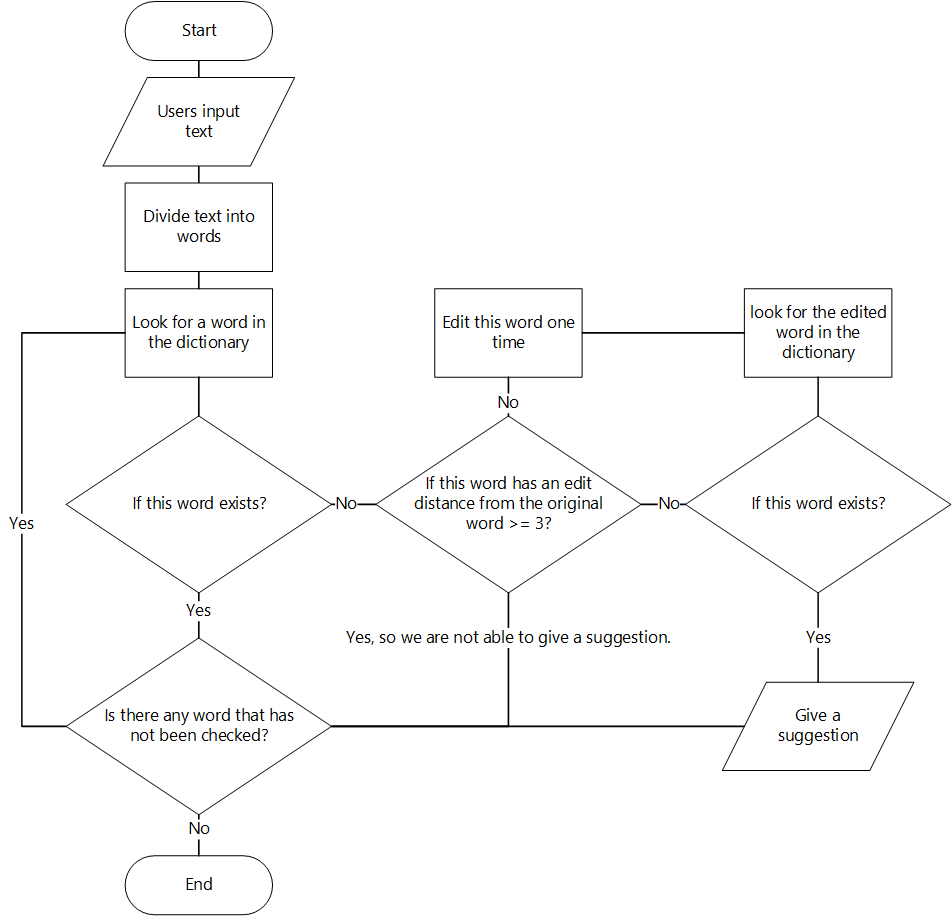
\includegraphics[width=0.5\textwidth]{fig/flow-diagram.png}
	\caption{Flow Diagram}
	\label{fig:flow-diagram}
\end{figure}
\item{ High Level Pseudo Code System Description. } \\
Pseudo codes are shown as follows.

\begingroup
\removelatexerror
\begin{algorithm}[H]
	\label{checkWord}
	\caption{checkWord}
	\KwData{Inputed text}
	\KwResult{Suggestions}
	split the input into words\;
	suggestions = an empty list of strings\;
	\ForEach{word in words}{
	suggestList = []\;
	\If{not checkDictionary(word)}{
		\For{i from 1 to 3}{
		\If{len(suggestList) $ > $ 5}{break;}
		editOneList = editDisOne(word)\;
		\ForEach{candidate in editOneList}{
			\If{len(suggestList) $ > $ 5}{break;}
			\If{checkDictionary (candidate)}{
				suggestList.append(candidate)\;
				suggestions[word] = suggestList\;
			}
		}
		}
	}
	}
	return suggestions\;
\end{algorithm}

\begin{algorithm}[H]
\label{checkDictionary}
\caption{checkDictionary}
\KwData{Word to be checked}
\KwResult{If this word is in dictionary}
	\eIf{word is in the ternary search tree}{
		return true;
	}{
		return false;
	}
\end{algorithm}

\begin{algorithm}[H]
\label{editDisOne}
\caption{editDisOne}
\KwData{Word to be edited}
\KwResult{A list of edited words}
splits = an empty list of pairs\;
deletes = an empty list of strings\;
transposes = an empty list of strings\;
replaces = an empty list of strings\;
inserts = an empty list of strings\;
result = an empty list of strings\;
\For{i from 1 to len(word) - 1}{splits.append([word(1, i), word(i + 1, len(word))])\;}
\ForEach{pair [a, b] in splits}{
	\If{len(b) $ > $ 1}{deletes.append(a + b(2, len(b)))\;}
	\If{len(b) $ > $ 2}{
		secondhalf = b(2, 2) + b(1, 1) + b(3, len(b))\;
		transposes.append(a + secondhalf)\;}
	\If{len(b) $ > $ 1}{
		\ForEach{letter in alphabet}{replaces.append(a + letter + b(2, len(b)))\;}
	}
	\ForEach{letter in alphabet}{replaces.append(a + letter + b(2, len(b)))\;}
}
put the candidates in deletes, transposes replaces and inserts into result\;
return result\;
\end{algorithm}
\endgroup

\item{Algorithms and Data Structures. } \\
In this project, we are using ternary search tree, which is a type of trie(or prefix tree). Compared to the 26-ary trie and binary tree, it has at most three children. So it's more space-efficient than trie. \\
Each node in ternary search tree stores a character, an indicator and up to three pointers pointing its children. The character is the data we stored. The indicator is a boolean value which tells us whether the node is the end of a word. The left child and the right child of the ternary seach tree act as the lowerbound and upperbound of prefix, help us easily find the prefix we actually want. \\
Ternary search tree supports tree operations: Insertion, search and deletion. The time complexity, as stated before, are $ O(\log n) $. \\
I also want to highlight the search operation. We process the string we want to search letter by letter. Everytime we try to look for only one letter in the ternary search tree. If the letter is equal to the character of current node, we move to the center child of current node and try to process next letter. If it is not, we move to the left or right child depending on the relation between the letter and the character of current node. The pseudo code is shown as Algorithm 4. \\
As Fig. 2 shows, it is a ternary search tree of word `TERNARY', `TREE', `TRIE' and `SEARCH'. 
\begin{figure}[H]
	\label{fig:tst}
	\centering
	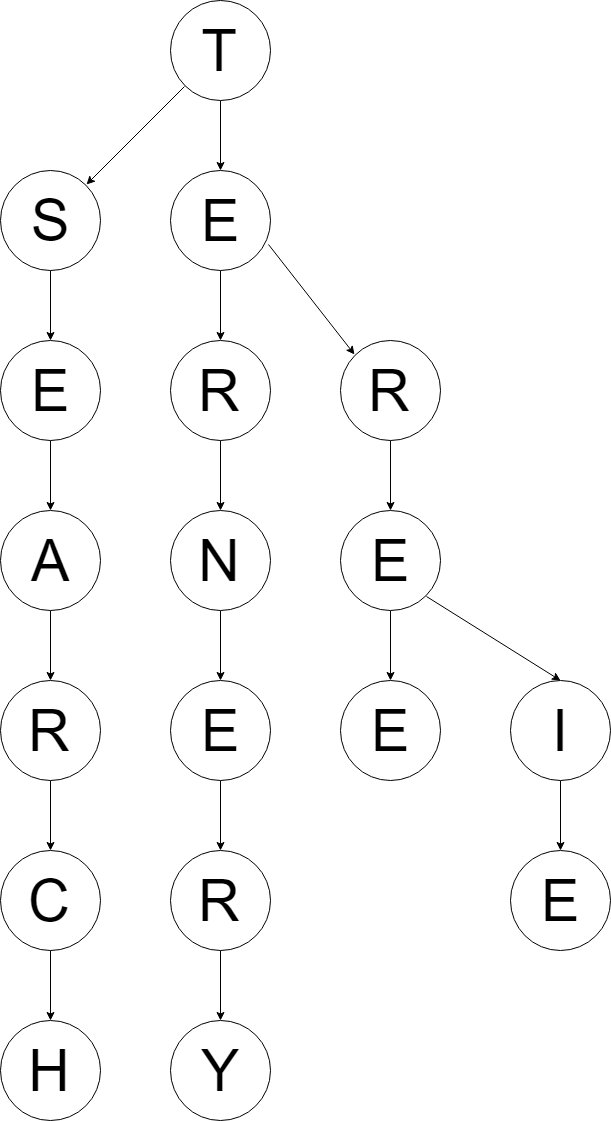
\includegraphics[height=0.3\textheight]{fig/TST.png}
	\caption{A ternary search tree}
\end{figure}

\begingroup
\removelatexerror
\begin{algorithm}[H]
	\label{search}
	\caption{Search in ternary search tree}
	\KwData{Word to be searched}
	\KwResult{Whether the search is successful}
	p $\gets$ the root of ternary search tree\;
	idx $\gets 0 $\;
	\While{p is not null}{
		\uIf{word[idx] $ < $ p.character}{
			p $\gets$ p.leftchild\;
		}
		\uElseIf{word[idx] $ > $ p.character}{
			p $\gets$ p.rightchild\;
		}
		\uElse {
			\If{idx == len(word) - 1 and p.indicator is true}{
				return true\;
			}
			idx $\gets$ idx + 1\;
			p $\gets$ p.centerchild
		}
	}
	return false\;
\end{algorithm}
\endgroup

\item{  Flow Diagram Major Constraints.}
Please insert here the integrity constraints:
\begin{itemize} 
\item{ Input Constraint: } \\
Description: In our project, we would check the spelling of English words, which means that the input must be English words, no matter if they are right or wrong. \\
Justification: All characters of each word inputed should be letters of alphabet. 
\end{itemize}
\end{itemize}


%
%\subsection{Stage3 - The Implementation Stage. }\label{sec: 3 The Implementation Stage.}
%%%%%%%%%%%%%%%%%%%%%%%%%%%%%%%%%%%%%%%%%%%%%%%%%%%%%%%%%%%%%%%%%%%%%%%%%%%%%%%%%%%%%%%%%%
%
We are using Python 3.7 as our programming languange for this project. 
The programming environment is as follows:
\paragraph{Operating System}{Ubuntu 18.04.1 LTS 64-bit}
\paragraph{Processor}{Intel$ ^\text{\textregistered} $ Core$ ^{\text{\texttrademark}} $ i7-8700K CPU}
\paragraph{Memory}{16 GB DDR4-3200 Memory}
\paragraph{Graphics Card}{GTX 1070ti} \\
%Building the corresponding relational tables, according to the proposed ER model described in the previous phase %enforcing the different integrity constraints.  
The deliverables for this stage include the following items:
\begin{itemize} 
\item{}
Sample small data snippet: \\
%The SQL tables that represent the ER project model, along with at least 3-5 rows of concrete data per table.
``Aoccdrnig to a rscheearch at Cmabrigde Uinervtisy, it deosn't mttaer in waht oredr the ltteers in a wrod are, the olny iprmoetnt tihng is taht the frist and lsat ltteer be at the rghit pclae. The rset can be a toatl mses and you can sitll raed it wouthit porbelm. Tihs is bcuseae the huamn mnid deos not raed ervey lteter by istlef, but the wrod as a wlohe.''
\item{}
Sample small output: \\
%The normalization steps for each table, along with explanations/justifications of each normalization step.
\textbf{If we choose the first suggestion in the list:} ``Aoccdrnig to a rscheearch at Cmabrigde Uinervtisy, it doesnt matter in what order the ltteers in a word are, the only iprmoetnt thing is that the frist and slat letter be at the grit place. The rest can be a total mess and you can still ared it outhit problem. his is abusee the human mind does not ared reve letter by istle, but the word as a wolve.'' \\
\textbf{If we choose the best suggestion in the list:} ``Aoccdrnig to a rscheearch at Cmabrigde Uinervtisy, it doesnt matter in what order the ltteers in a word are, the only iprmoetnt thing is that the frist and last letter be at the right place. The rest can be a total mess and you can still read it outhit problem. this is abusee the human mind does not read every letter by itself, but the word as a wolve.''
\item{}

Working code: \\
\textbf{The code of Trie (Ternary Search tree)} \\
\begin{minted}{python}
class Trie:
  root = None
  def __init__(self):
    self.root = None
  def insert(self, word):
    self.root = insert(self.root, word)
  def find(self, word):
    return find(self.root, word)

class Node:
  leftChild = None
  rightChild = None
  centerChild = None
  indicator = False
  character = None
  def __init__(self, character):
    self.character = character

def insert(node, word):
  if len(word) == 0:
    return node
  if node is None:
    node = Node(word[0])
  if word[0] < node.character:
    node.leftChild = insert(node.le
    ftChild, word)
  elif word[0] > node.character:
    node.rightChild = insert(node.r
    ightChild, word)
  else:
    if len(word[1:]) == 0:
      node.indicator = True
    else:
      node.centerChild = insert(n
      ode.centerChild, word[1:])
  return node

def find(node, word):
  if node is None or len(word) == 0:
    return False
  if word[0] < node.character:
    return find(node.leftChild, wor
    d)
  elif word[0] > node.character:
    return find(node.rightChild, wo
    rd)
  else:
    if len(word) == 1 and node.indi
    cator == True:
      return True
    return find(node.centerChild, w
    ord[1:])
\end{minted}
\textbf{The code of the checker:} \\
\begin{minted}{python}
def check_word(trie, word):
  suggest_list = []
  if check_dictionary(trie, word) == Fals
  e:
    edited_word_list = word
    for i in range(3):
      if len(suggest_list) >= 8:
        break
      edited_word_list = edit_word(ed
      ited_word_list, i + 1)
      for edited_word in edited_word_
      list:
        if edited_word in suggest_l
        ist:
          continue
        if len(suggest_list) >= 8:
          break
        if check_dictionary(trie, e
        dited_word) == True:
          suggest_list.append(edi
          ted_word)
    if len(suggest_list) == 0:
      suggest_list.append('No suggest
      ion')
  return suggest_list

def edit_word(word_or_list, edit_distance):
  if edit_distance <= 1:
    return edit_word_once(word_or_list)
  else:
    edited_list = []
    for edited_word in word_or_list:
      if len(edited_list) > 100000:
        break
      edited_list += edit_word_once(ed
      ited_word)
    return edited_list

def edit_word_once(word):
  splits = []
  delete_list = []
  traspose_list = []
  replace_list = []
  insert_list = []
  result = []
  for i in range(len(word) + 1):
    splits.append((word[0:i], word[i:]))
  for (a, b) in splits:
    if len(b) >= 1:
      delete_list.append(a + b[1:])
      for c in string.ascii_lowercase:
        replaced_word = a + c + b[1:]
        if word == replaced_word:
          continue
        replace_list.append(replaced_
        word)
    if len(b) >= 2:
      second_half = b[1] + b[0] + b[2:]
      traspose_list.append(a + second_h
      alf)
    for c in string.ascii_lowercase:
      insert_list.append(a + c + b)
  result = traspose_list + delete_list +
   replace_list + insert_list
  return result

def check_dictionary(trie, word):
  return trie.find(word)

def load_dictionary_from_json(filepath):
  with open(filepath) as dictionary_file:
    words = set(dictionary_file.read().spl
    it())
  return words

def load_dictionary_from_txt(filepath):
  with open(filepath) as dictionary_file:
    words = dictionary_file.readlines()
  return words

def load_dictionary_to_trie(words, trie):
  for word in words:
    trie.insert(word.strip())

def check_text(text):
  global trie_basic
  global trie_235k
  suggest_list_of_all_words = []
  for i in range(len(text)):
    suggest_list_of_all_words.append([])
    if text[i] in string.punctuation:
      continue
    print('Finding suggestions with respes
    ct to ' + text[i])
    if text[i] == 'i':
      suggest_list_of_all_words[i].appe
      nd('I')
      continue
    suggest_list_of_all_words[i] = check_w
    ord(trie_235k, text[i])
  print(suggest_list_of_all_words)
  return suggest_list_of_all_words
\end{minted}
%The SQL table after the normalization steps (showing all table attributes).
\item{}
Demo and sample findings
%The SQL statements used to create the SQL tables, including the required triggers as well as the integrity constraints. At %least 2 triggers and 2 of each of the following constraint types have to exist in the project tables overall: 
\begin{itemize} 
\item{}
	Data size: We have around 240,000 English vocabularies storing in a txt file of 2.5 MB. After fully loaded, the program takes around 300 MB of memory.
\item{}
	The accuracy of this program heavily depends on the vocabulary we have, and it is hard to do a perfect English spell checking system using merely Trie.
%Whether some users will be denied access and/or updates to some data according to their roles (for example: student1 %can not access other students' ' grades, so a violation error pops up upon that action. Another example: a sales person %can see an item price, but can not change it, since only a manger can, also a violation error pops up upon that update %attempt).
\end{itemize}
\end{itemize}


%
%\subsection{Stage4 -	User Interface. }\label{sec: 4. User Interface.}
%%%%%%%%%%%%%%%%%%%%%%%%%%%%%%%%%%%%%%%%%%%%%%%%%%%%%%%%%%%%%%%%%%%%%%%%%%%%%%%%%%%%%%%%%%%%%%%%%%%%%%%%%%%
%\textnormal{
Describe a User Interface (UI) to your application along with the related information that will be shown on each interface view (How users will query or navigate the data and view the query or navigation results). The emphasis should be placed on the process a user needs to follow in order to meet a particular information need in a user-friendly manner.
The deliverables for this stage include the following items :
}
\begin{itemize} 
\item{The modes of user interaction with the data (text queries, mouse hovering, and/or mouse clicks ?).} 
\item{The error messages that will pop-up when users access and/or updates are denied   }
\item{The information messages or results that wil pop-up in response to user interface events. }
	
\item{ The error messages in response to data range constraints violations.}
	
\item{ The interface mechanisms that activate different views in order to facilitate data accesses, according to users'  needs. }
	
\item{Each view created must be justified. Any triggers built upon those views should be explained and justified as well. At least one project view should be created with a justification for its use. }	
\end{itemize}

Please insert your deliverables for Stage4 as follows:
\begin{itemize} 
\item{The initial statement to activate your application with the corresponding initial UI screenshot}
	
\item{Two different  sample navigation user paths through the data exemplifying the different modes of interaction and the corresponding screenshots. }
\item{}
	The error messages popping-up when users access and/or updates are denied (along with explanations and examples):
	\begin{itemize} 
	\item{The error message: }
	\item{The error message explanation (upon which violation it takes place): }
	Please insert the error message explanation in here.
	\item{The error message example according to user(s) scenario(s): }
	Please insert the error message example in here.
	 \end{itemize}
\item{}
	The information messages or results that pop-up in response to user interface events.
	\begin{itemize} 
	\item{The information message: }
	Please insert the error message in here.
	\item{The information message explanation and the corresponding event trigger }
	\item{The error message example in response to data range constraints and the coresponding user's scenario }
	Please insert the error message example in here.
	 \end{itemize}
\item{}
	The  interface mechanisms that activate different views.
	\begin{itemize} 
	\item{The interface mechanism: }
	Please insert the interface mechanism here.
	 \end{itemize}
\end{itemize}


%
%\section{Project Highlights.}\label{sec:7. Project Highlights.}
%%%%%%%%%%%%%%%%%%%%%%%%%%%%%%%%%%%%%%%%%%%%%%%%%%%%%%%%%%%%%%%%%%%%%%%%%%%%%%%%%%%%%%%%%%%%%%%%%%%%%%%%%%%
%\textnormal{
\begin{itemize} 
\item{After we finished the project, we did an experiment using errors that are usually made by Wikipedia editors. We randomly chose 300 words from them, and our program made 70\% correct corrections.
(Data source: https://www.kaggle.com/bittlingmayer/spelling\#wikipedia.txt)}
\end{itemize}
}


\bibliographystyle{IEEEtran}
%\bibliography{IEEEabrv,bib_queyroi_abello2013}
%\bibliography{bib_queyroi_abello2013}

\end{document}


